\section{Desigualdades Clássicas}

Para iniciar, apresentamos algumas desigualdades simples mas famosas, válidas para quaisquer $a,b \in \R$:
\begin{itemize}
  \item $\modu a \ge 0$;
  \item $a^2 \ge 0$;
  \item $\modu {a+b} \le \modu a + \modu b$ (desigualdade triangular).
\end{itemize}

Essa última desigualdade, a chamada \emph{Desigualdade Triangular}, tem até em seu nome um apelo geométrico. Por que será que a chamamos de desigualdade triangular?

Antes de entender esse fato, chamo atenção para uma interpretação geométrica do módulo de um número real. 

Seja $x\in \R$ um número real qualquer. Podemos interpretar $\modu x$ como a distância de $x$ até a origem (ou zero) da reta dos números reais. Módulos e distâncias (ou comprimentos) tem uma relação intrínseca não só na reta, mas também no plano. Nesse ambiente, ao invés de tratarmos com números em uma reta, tratamos com vetores, representados por setas, cujos módulos coincidem exatamente com o seu comprimento. 

Tratar dos módulos desses elementos está além do escopo deste material. Mas, para entendermos o significado geométrico dessa desigualdade, vamos assumir que, dados dois vetores $a$ e $b$ no plano, o terceiro que com eles forma um triângulo é o vetor soma $a+b$. Levando isso em consideração, a desigualdade triangular, que diz que $$\modu {a+b} < \modu a +\modu b,$$ significa que o tamanho de qualquer um dos lados de um triângulo é menor que a soma do tamanho dos demais lados.

Na imagem abaixo, então, temos que são válidas as três desigualdades:
\begin{align*}
	a <  & b+c \\
    b <  & a+c \\
    c <  & a+b, 
\end{align*}

onde $a, b$ e $c$ são as medidas dos lados do triângulo.

\label{fig:destri1}
\begin{figure}[H]
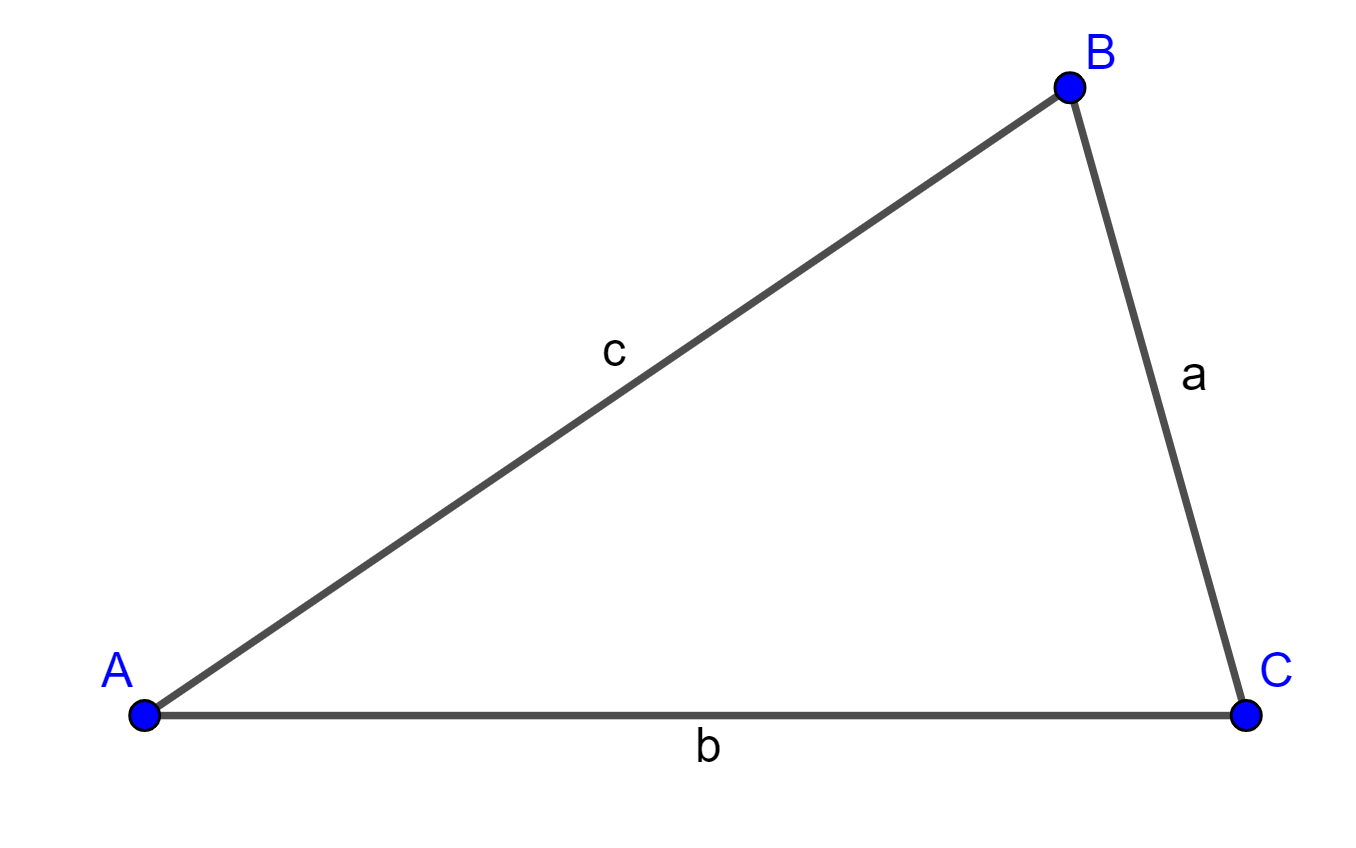
\includegraphics[scale=0.25]{\imgdirfromsection/DesTriang1.png}
\centering
\end{figure}

Para verificar que, de fato, essas desigualdades devem ser satisfeitas em um triângulo, vamos levar em consideração o maior lado do triângulo acima e traçar circulos centrados em cada uma de suas extremidades de modo que a soma dos raios seja menor que o comprimento do lado em questão.

\label{fig:destri2}
\begin{figure}[H]
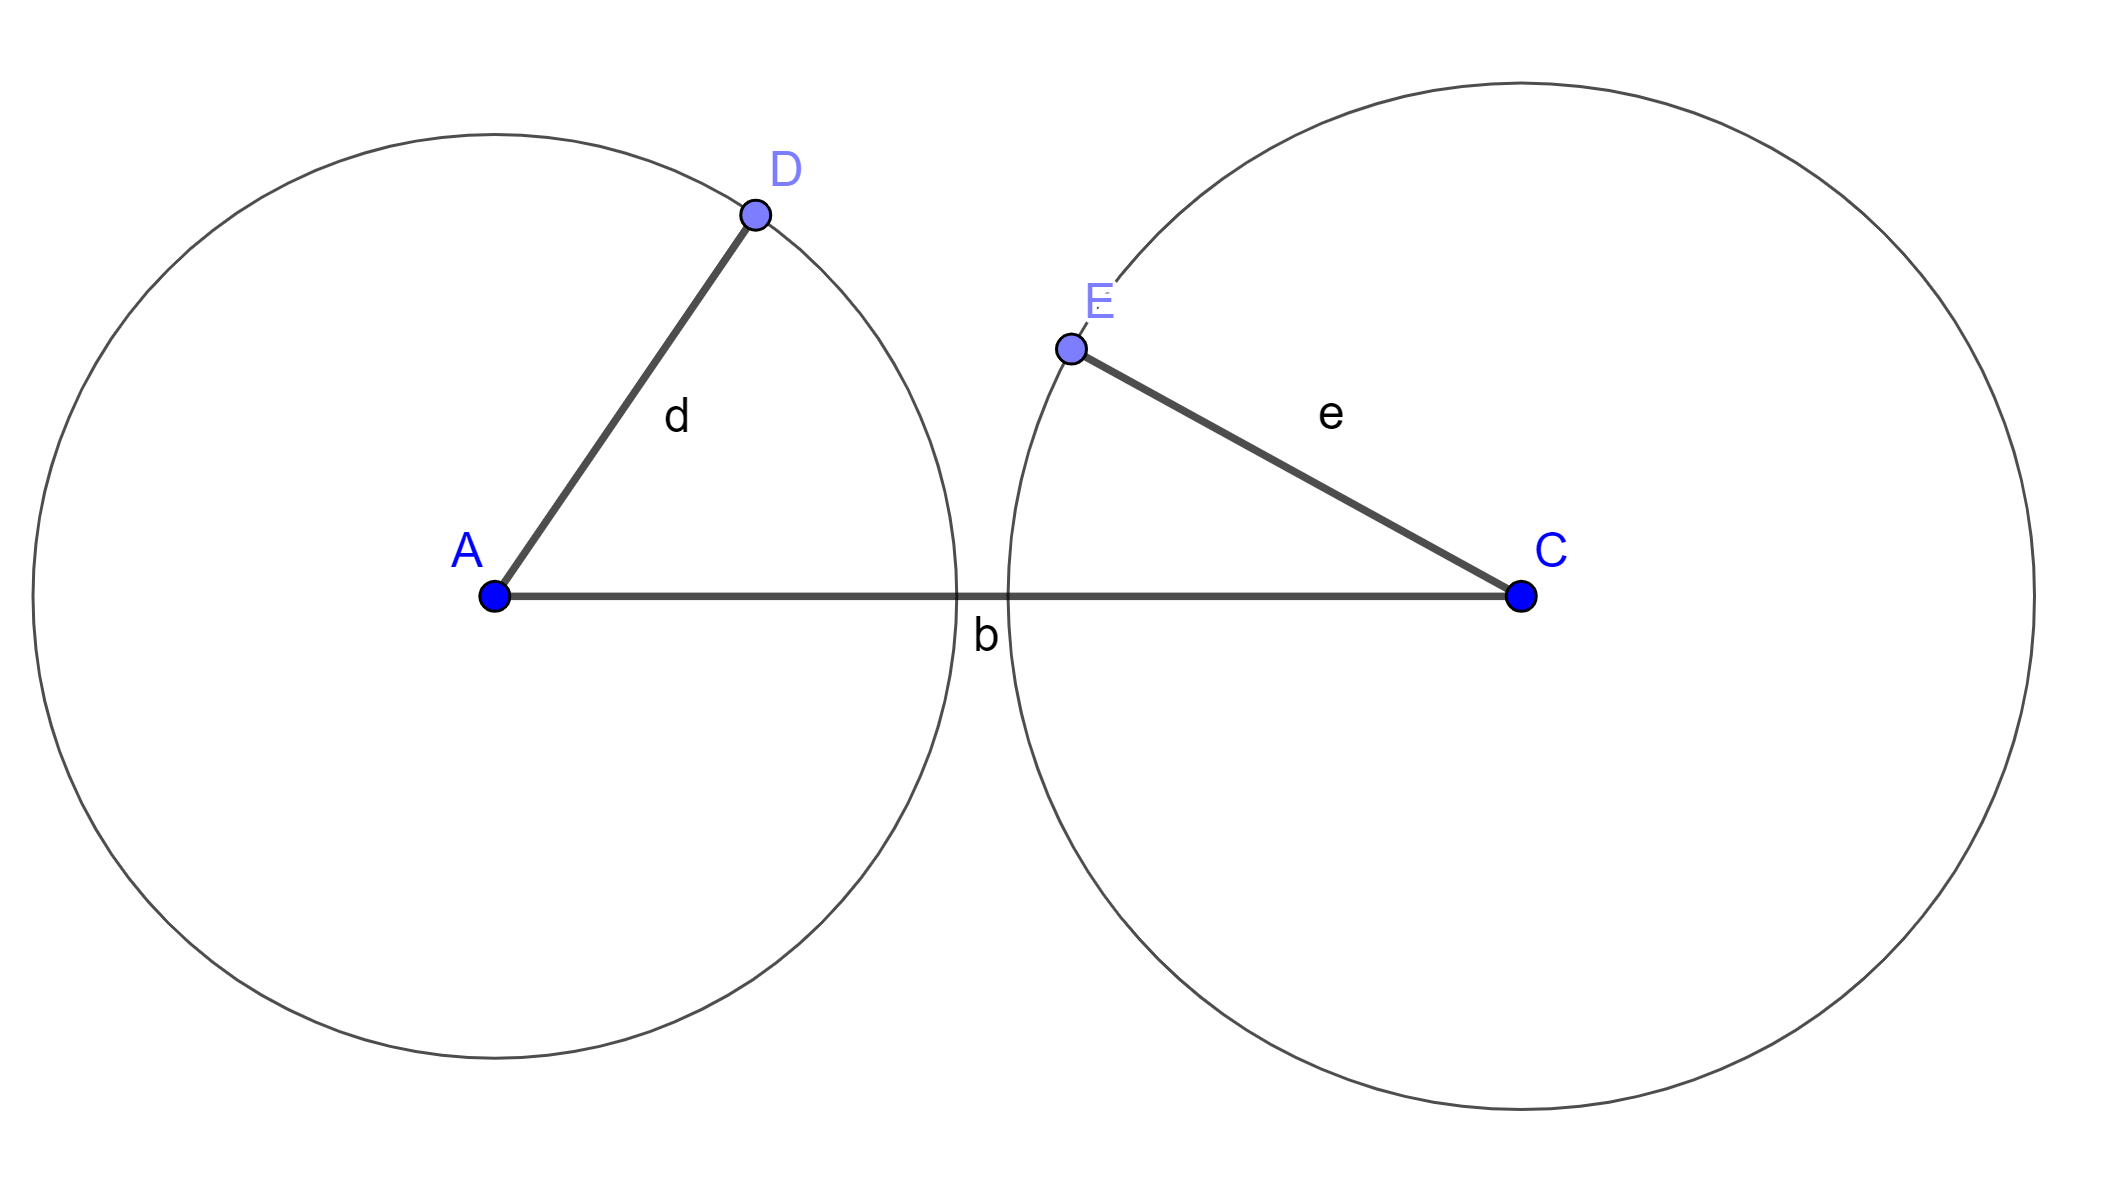
\includegraphics[scale=0.25]{\imgdirfromsection/DesTriang2.png}
\centering
\end{figure}

Note que quaisquer dois segmentos partindo de $A$ e de $C$, cuja soma dos comprimentos seja menor que o comprimento do segmento $AC$ não poderão formar com $AC$ um triangulo. Na imagem, temos $d+e < b$ e, portanto, não é possível ter um triângulo.


\begin{theorem}
\label{theorem:ineq-prod-quad}
Para quaisquer $x, y \in \R$, vale:
%
\begin{equation*}
    xy \le \frac {x^2 +y^2} 2.
\end{equation*}
%
Além disso, a igualdade acontece se, e somente se, $x=y$.
\end{theorem}

\begin{proof}
Sejam $x, y \in \R$. Sabemos que $(x-y)^2 \ge 0$. Segue que:
%
\begin{align*}
	(x-y)^2 \ge 0 \iff & x^2 - 2xy + y^2 \ge 0 \\
				  \iff & 2xy \le x^2 + y^2 \\
				  \iff & xy \le \frac {x^2 + y^2} 2
\end{align*}
%
Ademais, note que a igualdade $xy = \frac {x^2 + y^2} 2$ ocorre quando:
%
\begin{align*}
	xy = \frac {x^2 + y^2} 2 \iff & (x-y)^2 = 0 \\
							 \iff & x-y = 0 \\
							 \iff & x = y
\end{align*}
\end{proof}

\begin{theorem}
\label{theo:desigualdade-medias-dois-termos}
Para quaisquer $a, b \in \R_+$, vale:
%
\begin{equation*}
    \sqrt{ab} \leq \frac {a +b} 2.
\end{equation*}
Além disso, a igualdade acontece se, e somente se, $a=b$.
\end{theorem}

\begin{proof}
Sejam $a, b \in \R_+$. Para provar o teorema, basta aplicar o Teorema \ref{theorem:ineq-prod-quad} com $x = \sqrt a$ e $y = \sqrt b$.
\end{proof}

\begin{theorem}[Desigualdade das médias aritmética e geométrica]
\label{theorem:ineq-avg-ari-geo}
Para quaisquer $n \in \nnats$ e $a_1, a_2, \dots , a_n \in \R_+$, vale:
%
\begin{equation*}
    \sqrt[n]{a_1\dots a_n} \leq \frac {a_1 + \dots + a_n} n.
\end{equation*}
\end{theorem}

\begin{theorem}[Desigualdade das médias harmônica e geométrica]
Para quaisquer $n \in \nnats$ e $a_1, a_2, \dots , a_n \in \R_+^*$, vale:
%
\begin{equation*}
    \frac n {\frac 1 {a_1} + \dots + \frac 1 {a_n}}  \leq \sqrt[n]{a_1\dots a_n}  .
\end{equation*}
\end{theorem}

\begin{proof}
Sejam $a_1, a_2, \dots, a_n \in \R_+ ^*$. Considere $b_i = \frac 1 {a_i}$ para todo $i \in \set{1, 2, \dots, n}$. Usando o Teorema \ref{theorem:ineq-avg-ari-geo} com todos os $b_i$, tem-se que:
%
\begin{eqnarray*}
\sqrt[n]{b_1 \cdot \dots \cdot b_n } \le \frac {b_1 + \dots + b_n } n & \iff \frac n {b_1 + \dots + b_n } & \le \frac 1 {\sqrt[n]{b_1 \cdot \dots \cdot b_n }} \\
& \iff \frac n {\frac 1 {a_1} + \dots + \frac n {a_n}} & \le \frac 1 {\sqrt[n]{\frac 1 {a_1 \cdot \dots \cdot a_n}}} \\ 
& & = \frac 1 {\frac 1 {\sqrt[n]{a_1 \cdot \dots \cdot a_n}}} \\ 
& & =  \sqrt[n]{a_1 \cdot \dots \cdot a_n}
\end{eqnarray*}
\end{proof}

\begin{theorem}[Desigualdade de Cauchy-Schwarz]
Sejam $x_1, \dots , x_n, y_1, \dots y_n \in \R$. O seguinte vale:
%
\begin{equation*}
    \modu{x_1y_1 + \dots + x_ny_n} \leq \sqrt{x^2_1+ \dots + x^2_n}
    \cdot \sqrt{y^2_1+ \dots + y^2_n}.
\end{equation*}
%
Além disso, a igualdade só ocorre se existir um número real $\alpha$ tal que $x_1 = \alpha y_1$, ..., $x_n = \alpha y_n$.
\end{theorem}

\begin{example}
Duas torres são amarradas por uma corda $APB$ que vai do topo $A$ da primeira torre para um ponto $P$ no chão, entre as torres, e então
até o topo $B$ da segunda torre. Qual a posição do ponto $P$ que nos dá o comprimento mínimo da corda a ser utilizada?
\end{example}

\begin{solution}
Tomando $B'$ como o reflexo de $B$ em relação ao chão, conforme a Figura \ref{fig:torres}, temos que o comprimento da corda $\overline{AP} + \overline{PB}$ é igual a $\overline{AP} + \overline{PB'}$. 

\label{fig:torres}
\begin{figure}[H]
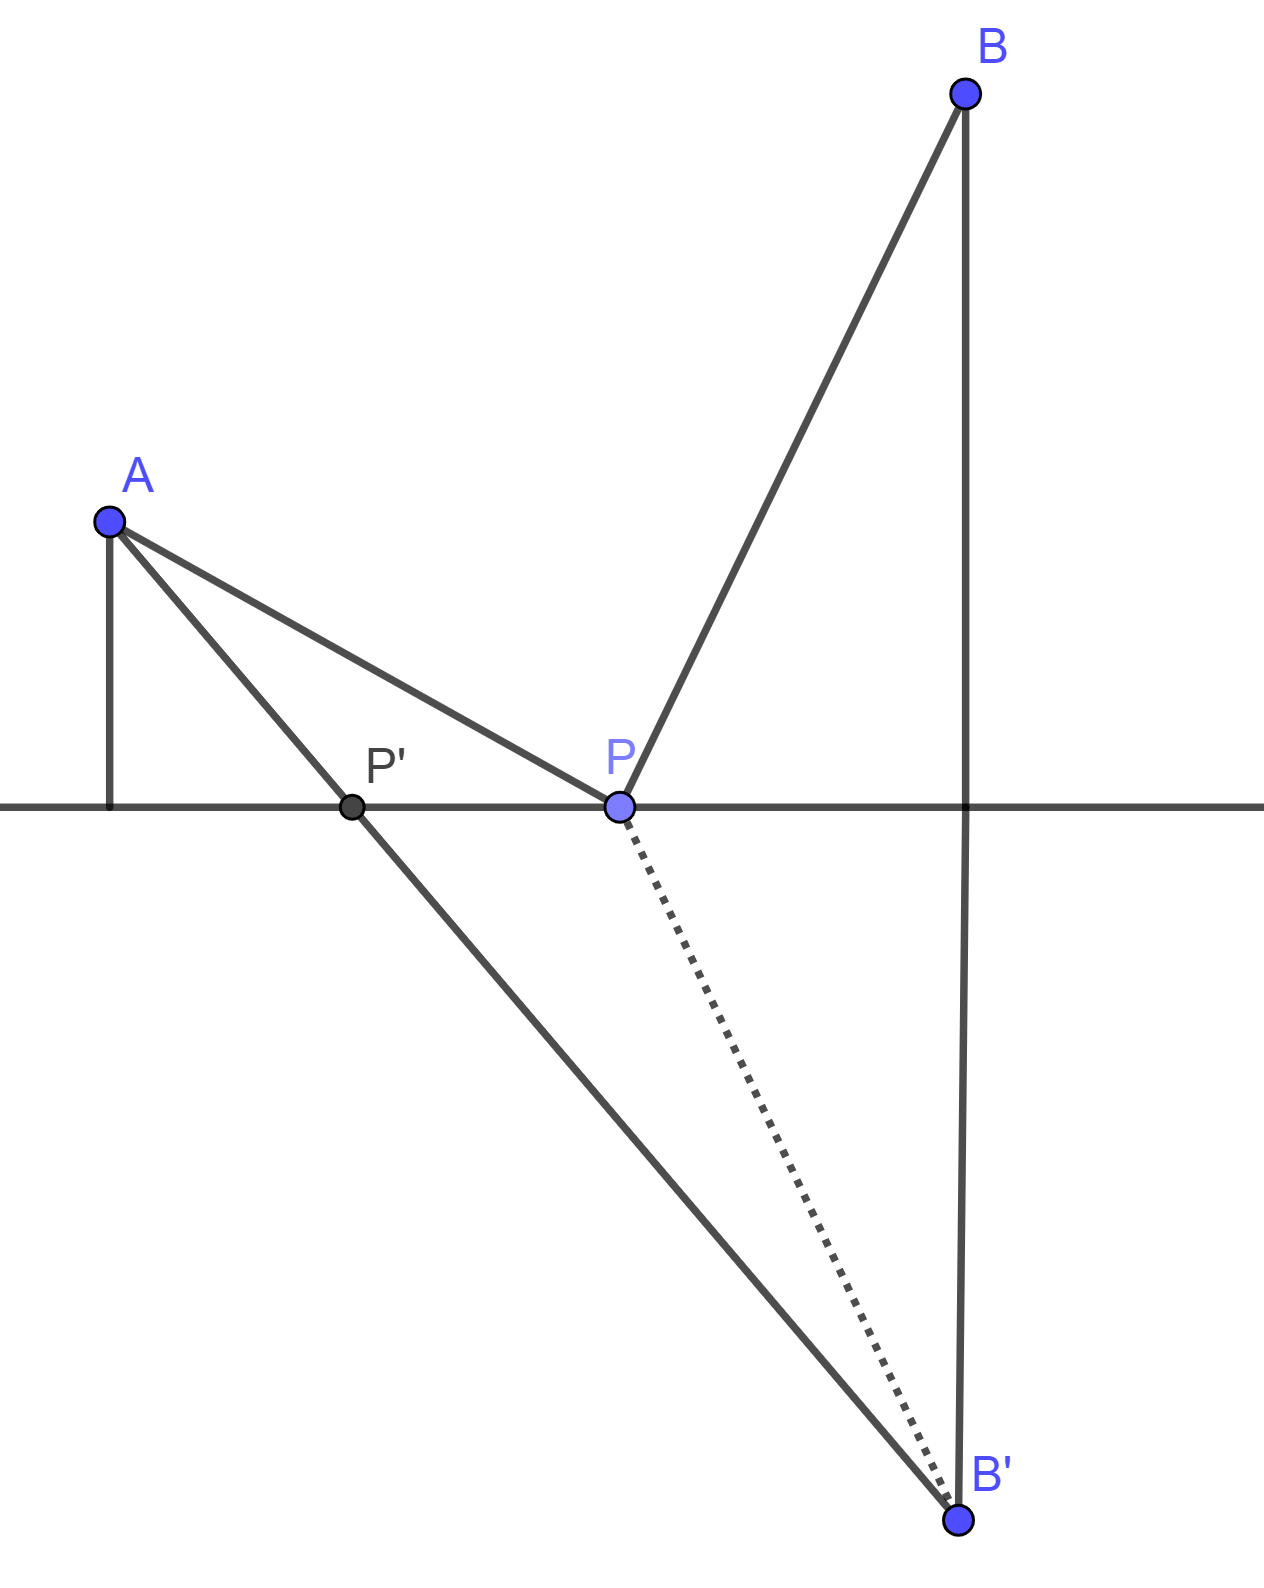
\includegraphics[scale=0.25]{\imgdirfromsection/fig-c03-ex29.png}
\centering
\end{figure}

Traçando $AB'$ e tomando $P'$ como a interseção de $AB'$ com o chão, tem-se que $P'$ é a solução do problema pois, pela desigualdade triangular, segue que:
%
\begin{align*}
\overline{AP'} +\overline{P'B} & = \overline{AP'} +\overline{P'B'} \\
& = \overline{AB'} \\
& \le \overline{AP} +\overline{PB'} \\
& = \overline{AP} +\overline{PB} 
\end{align*}
%
Logo, $\overline{AP'} +\overline{P'B} \le \overline{AP} +\overline{PB}$.
\end{solution}

\begin{example}
Prove que, num triângulo retângulo, a altura relativa à hipotenusa é sempre menor ou igual que a metade da hipotenusa. Prove, ainda, que
a igualdade só ocorre quando o triângulo retângulo é isósceles.
\end{example}

\begin{solution}
Considere um triângulo retângulo como o da Figura \ref{fig:rect-triangle}.
%
\label{fig:rect-triangle}
\begin{figure}[H]
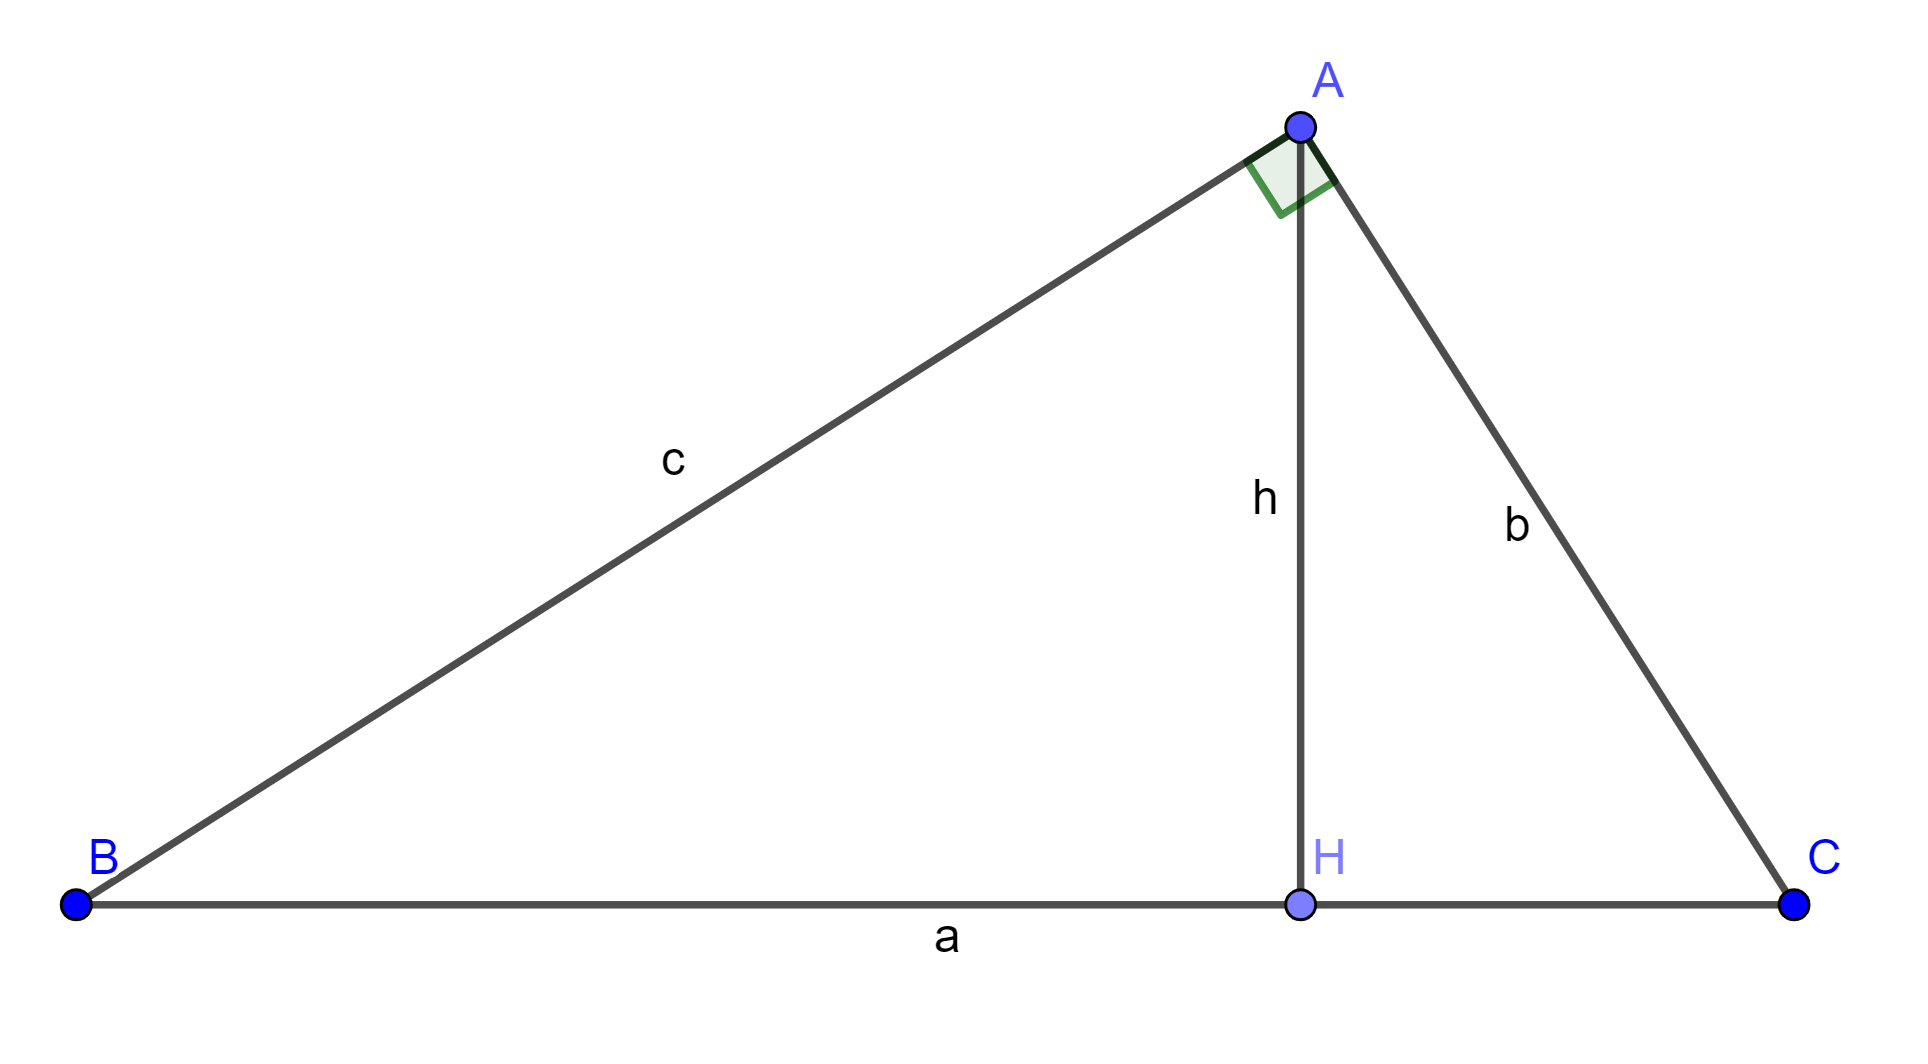
\includegraphics[scale=0.25]{\imgdirfromsection/03-triangle.png}
\centering
\end{figure}
%
Queremos provar que $h \le \frac a 2$. Da semelhança entre $AHC$ e $BAC$, segue que:
%
\begin{equation*} 
\frac b h = \frac a c \iff ah = bc
\end{equation*} 
%
Do Teorema \ref{theorem:ineq-prod-quad}, segue que:
%
\begin{align*}
ah = bc \le \frac {b^2 + c^2} 2 = \frac {a^2} 2,
\end{align*}
%
ou seja, 
%
\begin{align*}
ah \le \frac {a^2} 2 \iff h \le \frac a 2.
\end{align*}
%
Além disso, a igualdade só será válida quando $b=c$, ou seja, quando o triângulo for isósceles.
\end{solution}

\begin{example}
Prove que, entre todos os triângulos retângulos de catetos $a$ e $b$, e com hipotenusa $c$ fixada, o que tem maior soma dos catetos
$S = a+b$ é o triângulo isósceles.
\end{example}

\begin{solution}
Seja um triângulo retângulo com hipotenusa $c$ fixada e catetos $a$ e $b$. Utilizando a Desigualdade de Cauchy-Schwarz com $x_1 = a$, $x_2 = b$, $y_1 = 1$ e $y_2 = 1$, temos que:
%
\begin{align*}
\modu {a \cdot 1 + b \cdot 1} \le \sqrt{a^2 + b^2} \cdot \sqrt{1^2 + 1^2} \iff S = a+b \le c\sqrt 2.
\end{align*}
%
Além disso, da Desigualdade, segue que $S$ é igual a $c\sqrt 2$, ou seja, atinge seu valor máximo se, e somente se, $a = \alpha \cdot 1$ e $b = \alpha \cdot 1$ para certo $\alpha \in \R$. Logo, o triângulo deve ser isósceles, com $a=b$.
\end{solution}